%%%%%%%%%%%%%%%%%%%%%%%%%%%%%%%%%%%%%%%%%%%%%%%%%%%%%%%%%%%%%%%%%%%%%%
%%  Copyright by Wenliang Du.                                       %%
%%  This work is licensed under the Creative Commons                %%
%%  Attribution-NonCommercial-ShareAlike 4.0 International License. %%
%%  To view a copy of this license, visit                           %%
%%  http://creativecommons.org/licenses/by-nc-sa/4.0/.              %%
%%%%%%%%%%%%%%%%%%%%%%%%%%%%%%%%%%%%%%%%%%%%%%%%%%%%%%%%%%%%%%%%%%%%%%

\newcommand{\commonfolder}{../../common-files}

\documentclass[11pt]{article}

\usepackage[most]{tcolorbox}
\usepackage{times}
\usepackage{epsf}
\usepackage{epsfig}
\usepackage{amsmath, alltt, amssymb, xspace}
\usepackage{wrapfig}
\usepackage{fancyhdr}
\usepackage{url}
\usepackage{verbatim}
\usepackage{fancyvrb}
\usepackage{adjustbox}
\usepackage{listings}
\usepackage{color}
\usepackage{subfigure}
\usepackage{cite}
\usepackage{sidecap}
\usepackage{pifont}
\usepackage{mdframed}
\usepackage{textcomp}
\usepackage{enumitem}
\usepackage{hyperref}


% Horizontal alignment
\topmargin      -0.50in  % distance to headers
\oddsidemargin  0.0in
\evensidemargin 0.0in
\textwidth      6.5in
\textheight     8.9in 

\newcommand{\todo}[1]{
\vspace{0.1in}
\fbox{\parbox{6in}{TODO: #1}}
\vspace{0.1in}
}


\newcommand{\unix}{{\tt Unix}\xspace}
\newcommand{\linux}{{\tt Linux}\xspace}
\newcommand{\minix}{{\tt Minix}\xspace}
\newcommand{\ubuntu}{{\tt Ubuntu}\xspace}
\newcommand{\setuid}{{\tt Set-UID}\xspace}
\newcommand{\openssl} {\texttt{openssl}}


\pagestyle{fancy}
\lhead{\bfseries SEED Labs}
\chead{}
\rhead{\small \thepage}
\lfoot{}
\cfoot{}
\rfoot{}


\definecolor{dkgreen}{rgb}{0,0.6,0}
\definecolor{gray}{rgb}{0.5,0.5,0.5}
\definecolor{mauve}{rgb}{0.58,0,0.82}
\definecolor{lightgray}{gray}{0.90}


\lstset{%
  frame=none,
  language=,
  backgroundcolor=\color{lightgray},
  aboveskip=3mm,
  belowskip=3mm,
  showstringspaces=false,
%  columns=flexible,
  basicstyle={\small\ttfamily},
  numbers=none,
  numberstyle=\tiny\color{gray},
  keywordstyle=\color{blue},
  commentstyle=\color{dkgreen},
  stringstyle=\color{mauve},
  breaklines=true,
  breakatwhitespace=true,
  tabsize=3,
  columns=fullflexible,
  keepspaces=true,
  escapeinside={(*@}{@*)}
}

\newcommand{\newnote}[1]{
\vspace{0.1in}
\noindent
\fbox{\parbox{1.0\textwidth}{\textbf{Note:} #1}}
%\vspace{0.1in}
}


%% Submission
\newcommand{\seedsubmission}{
Debe enviar un informe de laboratorio detallado, con capturas de pantalla, para describir lo que ha hecho y lo que ha observado.
También debe proporcionar una explicación a las observaciones que sean interesantes o sorprendentes.
Enumere también los fragmentos de código más importantes seguidos de una explicación. No recibirán créditos aquellos fragmentos de códigos que no sean explicados.}

%% Book
\newcommand{\seedbook}{\textit{Computer \& Internet Security: A Hands-on Approach}, 2nd
Edition, by Wenliang Du. Para más detalles \url{https://www.handsonsecurity.net}.\xspace}

%% Videos
\newcommand{\seedisvideo}{\textit{Internet Security: A Hands-on Approach},
by Wenliang Du. Para más detalles \url{https://www.handsonsecurity.net/video.html}.\xspace}

\newcommand{\seedcsvideo}{\textit{Computer Security: A Hands-on Approach},
by Wenliang Du. Para más detalles \url{https://www.handsonsecurity.net/video.html}.\xspace}

%% Lab Environment
\newcommand{\seedenvironment}{Este laboratorio ha sido testeado en nuestra imagen pre-compilada de una VM con Ubuntu 16.04, que puede ser descargada del sitio oficial de SEED.\xspace}

\newcommand{\seedenvironmentA}{Este laboratorio ha sido testeado en nuestra imagen pre-compilada de una VM con Ubuntu 16.04, que puede ser descargada del sitio oficial de SEED.\xspace}

\newcommand{\seedenvironmentB}{Este laboratorio ha sido testeado en nuestra imagen pre-compilada de una VM con Ubuntu 20.04, que puede ser descargada del sitio oficial de SEED .\xspace}

\newcommand{\seedenvironmentC}{Este laboratorio ha sido testeado en nuestra imagen pre-compilada de una VM con Ubuntu 20.04, que puede ser descargada del sitio oficial de SEED. Sin embargo, la mayoría de nuestros laboratorios pueden ser realizados en la nube para esto Ud. puede leer nuestra guía que explica como crear una VM de SEED en la nube.\xspace}

\newcommand{\seedenvironmentAB}{
Este laboratorio ha sido testeado en nuestras imagenes pre-compiladas de una VM con Ubuntu 16.04 y otra con Ubuntu 20.04, que pueden ser descargadas del sitio oficial de SEED.\xspace}

\newcommand{\nodependency}{Dado que utilizamos contenedores para configurar el entorno de laboratorio, este laboratorio no depende estrictamente de la VM de SEED. Puede hacer este laboratorio utilizando otras máquinas virtuales, máquinas físicas o máquinas virtuales en la nube.\xspace}

\newcommand{\adddns}{You do need to add the required IP address mapping to
the \texttt{/etc/hosts} file.\xspace}






\newcommand{\seedlabcopyright}[1]{
\vspace{0.1in}
\fbox{\parbox{6in}{\small Copyright \copyright\ {#1}\ \ by Wenliang Du.\\
      Este trabajo se encuentra bajo licencia Creative Commons.
       Attribution-NonCommercial-ShareAlike 4.0 International License.
       Si ud. remezcla, transforma y construye a partir de este material,
       Este aviso de derechos de autor debe dejarse intacto o reproducirse de una manera que sea razonable para el medio en el que se vuelve a publicar el trabajo.
       }}
\vspace{0.1in}
}






\usepackage{longtable}
\usepackage{enumitem}
\usepackage{stackengine}
\newcommand\xrowht[2][0]{\addstackgap[.5\dimexpr#2\relax]{\vphantom{#1}}}



\newcommand{\miniVPN}{{\tt MiniVPN}\xspace}
\newcommand{\hostu}{{\tt U}\xspace}
\newcommand{\hostv}{{\tt V}\xspace}


\newcommand{\vpnFigs}{./Figs}

\lhead{\bfseries SEED Labs -- Laboratorio de VPN}


\begin{document}

\begin{center}
{\LARGE Laboratorio de VPN}
\end{center}

\seedlabcopyright{2006 - 2016}



% *******************************************
% SECTION
% ******************************************* 
\section{Descripción}

Una Virtual Private Network (VPN) o Red Privada Virtual se usa para crear un ámbito privado de comunicación entre computadoras o para proveer ua extensión segura de una red privada dentro de una red insegura tal como Internet. VPN es una tecnología ampliamente usada. Una VPN puede ser construída sobre IPSec o TLS/SSL (Transport Layer Security/Secure Socket Layer). 
Son dos estrategias diferentes para construir VPNs. En este laboratorio, nos centramos en VPNs basadas en  TLS/SSL. Este tipo de VPNs son conocidas como VPNs TLS/SSL.

El objetivo de este laboratorio es que los estudiantes profundizen los conocimientos en redes y las tecnologías que hacen seguras a las VPNs. Para lograr este cometido, se les pedirá a los estudiantes que implementen una VPN TLS/SSL simple.
Aunque esta VPN es sencilla, esta cinluya todos los elementos esenciales de una VPN. El diseño y la implementación de una VPN TLS/SSL ejemplifican
una serie de principios de seguridad, incluídos los siguientes:

\begin{itemize}[noitemsep]
\item Virtual Private Network (VPN)
\item TUN/TAP y IP tunneling 
\item Enrutamiento
\item Certificados Public-key cryptography, PKI, y X.509 
\item Programación TLS/SSL
\item Autenticación
\end{itemize}


\paragraph{Lecturas y Videos.}
Para una cobertura más detallada sobre VPN, PKI, y TLS puede consultar:

\begin{itemize}
\item Capítulos 19, 24, y 25 de libro de SEED, \seedbook
\item Sección 8 del curso de SEED en Udemy, \seedisvideo
\end{itemize}


\paragraph{Laboratorios Relacionados.}
Tenemos un laboratorio separado sobre PKI y otro sobre TLS. Se recomienda a los estudiantes terminar esos laboratorios de criptografía antes de empezar a trabjar con este laboratorio. Si los estudiantes están solamente interesados en la sección de VPN Tunneling (sin incluir la parte de criptografía), deberían de consultar el laboratario de VPN Tunneling en su lugar, en vez de este.

\paragraph{Entorno de Laboratorio.} 
\seedenvironmentB
Necesitamos usar el paquete \openssl en este laboratorio. Este paquete incluye los archivos de encabezado, librerías y comandos. Este paquete está instalado en nuestra imagen de la Máquina Virtual.




\newpage
% *******************************************
% SECTION
% ******************************************* 
\section{Tareas del Laboratorio}

En este laboratorio, los estudiantes deberán de implementar una VPN simple para \linux. La llamaremos {\tt miniVPN}. 


% -------------------------------------------
% SUBSECTION
% ------------------------------------------- 
\subsection{Tarea 1: Setup de la Máquina Virtual}

Crearemos un Túnel VPN entre la máquina cliente y el gateway, permitiéndole a la máquina el acceso seguro a la red privada a través del gateway.
Necesitaremos al menos tres Máquinas Virtuales: el cliente VPN (también usado como Host U), el servidor VPN (gateway), y el host en la red privada (Host V).
El setup de esta red es ilustrado en la Figura \ref{vpn:fig:host2gateway}.

\begin{figure}[htb]
\begin{center}
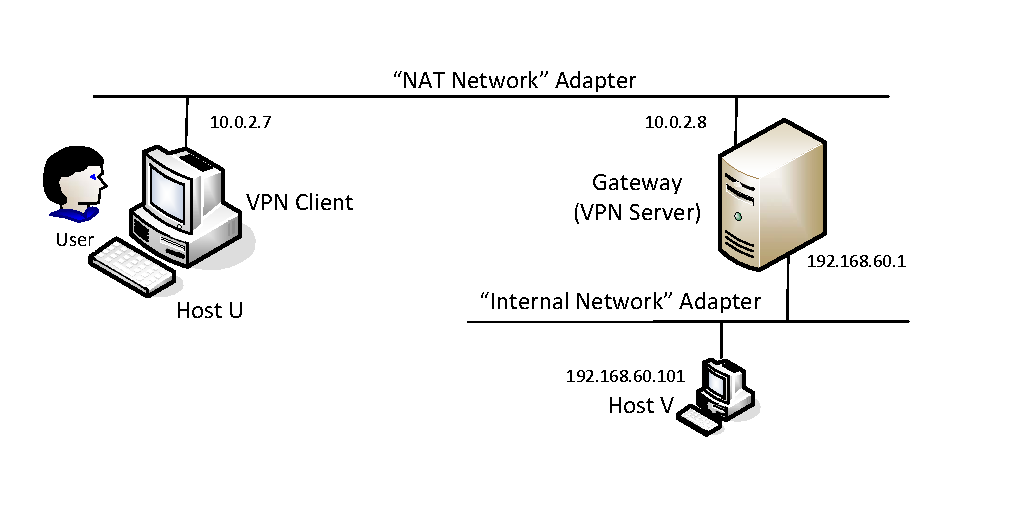
\includegraphics[width=0.9\textwidth]{\vpnFigs/Host2Gateway.pdf}
\end{center}
\caption{VM setup for this lab}
\label{vpn:fig:host2gateway}
\end{figure}
 

En la práctiva, el cliente VPN y el servidor VPN estarán conectados vía Internet.
Para no complicar las cosas, conectaremos estas dos máquinas a la misma LAN, es decir la LAN simulará la Internet.
Usaremos el adaptador ``NAT Network'' para esta LAN.
La tercera máquina, Host V, es una máquina dentro de la red privada. Los usuarios en el Host U (fuera de la red privada) quieren comunicarse con el Host V usando el Túnel VPN. Para simular esta configuración, conectaremos el Host V al servidor VPN (también será el gateway) a través de una  ``Internal Network''. En este escenario de configuración, el Host V no es accesible directamente desde Internet; o desde el Host U.

Note que si una máquina virtual usa el modo ``Internal Network'', VirtualBox no ofrece DHCP a esta, por lo que la máquina virtual debe ser configurada de forma estática. Para hacer esto haga click en el ícono de network en la esquina derecha superior del escritorio y seleccione \texttt{"Edit Connections"}. Verá una lista de \texttt{"Wired connections"}, una por cada adaptador de red usado por la máquina virtual.
Para el Host V, hay sólo una conexión pero para el servidor VPN, usaremos dos. Para asegurarse que ud. seleccione el adaptador que corresponde al adaptador de ``Internal Network'', puede chequear la dirección MAC mostrada en el pop-up después de haber elejido editar la conexión.
Compare esta dirección MAC con la que ud. obtiene de  \texttt{ifconfig}, y así sabrá si es la correcta o no.

Después de haber seleccionado la conexión que se debe de editar, seleecione el tab que dice \texttt{"ipv4 Settings"} y elija el método Manual, en vez del que se usa por defecto que es \texttt{"Automatic (DHCP)"}. Haga click en el botón de \texttt{"Add"}  para configurar la dirección IP para la máquina virtual. Para más detalles vea la Figura  \ref{vpn:fig:internalnetwork}.



\begin{figure}[htb]
\begin{center}
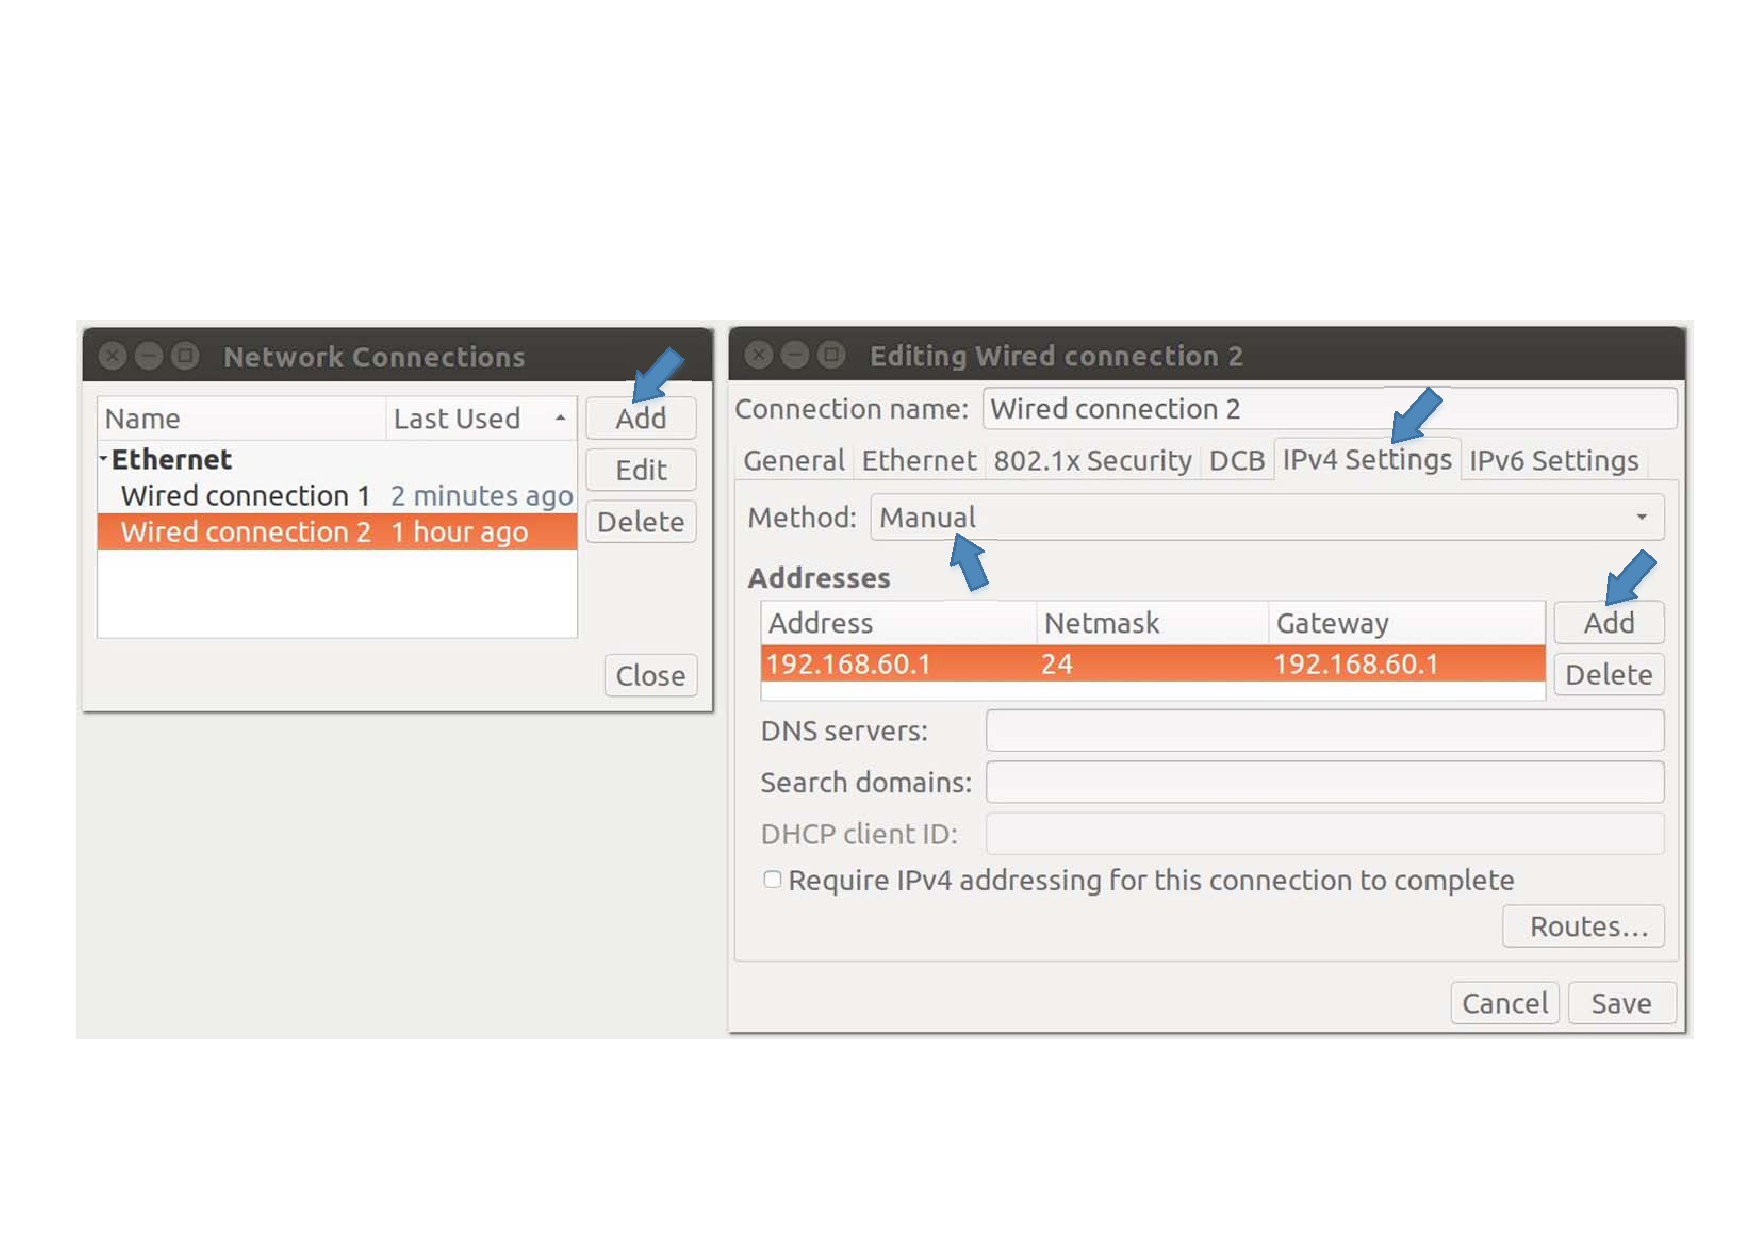
\includegraphics[width=0.8\textwidth]{\vpnFigs/InternalNetwork.pdf}
\end{center}
\caption{Configuración Manual de la IP para el adaptador \texttt{"Internal Network"} del servidor VPN.}
\label{vpn:fig:internalnetwork}
\end{figure}
 


% -------------------------------------------
% SUBSECTION
% ------------------------------------------- 
\subsection{Tarea 2: Creando un Túnel VPN usando TUN/TAP}

Activar la tecnología para las VPNs TLS/SLL es TUN/TAP, las cuales son ampliamente implementadas en los sistemas operativos modernos.
TUN y TAP son drivers del kernel de redes virtuales; implementan un dispositivo de red que es soportado por el software.
TAP simula un dispositivo ethernet y opera con paquetes de capa 2 como lo son los Frames de Ethernet; TUN simula un dispositivo de capa red y opera con paquetes de capa 3 como lo son los paquetes IP.
Con TUN/TAP, podemos crear interfaces de red virtuales.

Un programa en el espacio de usuario está frecuentemente ligado a una interfaz de red virtual TUN/TAP.
Los paquetes enviados por el sistema operativo usando la interfaz de red TUN/TAP son entregados al programa en espacio de usuario. Por otro lado los paquetes enviados por el programa usando la interfaz de red TUN/TAP son inyectados dentro del stack de red del sistema operativo, y hace parecer que los paquetes provienen de un origen externo a través de la interfaz de red virtual.

Cuando un programa se liga a la interfaz TUN/TAP, los paquetes IP que envía la máquina a esta interfaz serán canalizados dentro del programa; por otro lado, los paquetes IP que el programa envía a la interfaz serán canalizados dentro de la máquina, como si ellos hubieran venido de afuera de la red a través de esta red de interfaz virtual. El programa puede usar las llamadas al sistema estandar  {\tt read()} y {\tt write()} para recibir estos paquetes desde la interfaz virtual o para enviarlos a través de la misma.

Hemos creado un cliente VPN de ejempolo llamado (\texttt{vpnclient}) y un servidor  (\texttt{vpnserver}), ambos pueden ser descargados del sitio oficial del laboratorio.
Los programas son explicados en detalle en el Capítulo 16 del libro de SEED llamado \textit{Computer \& Internet Security: A Hands-on Approach, 2nd Edition}; este Capítulo también explica como funciona TUN/TAP y como usarlos para crear una VPN.


\begin{figure}[htb]
\begin{center}
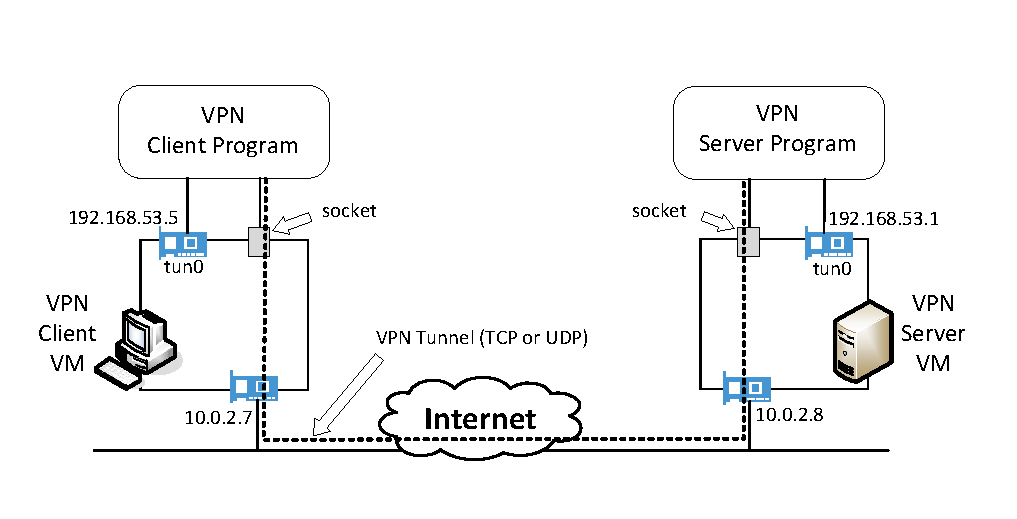
\includegraphics[width=0.9\textwidth]{\vpnFigs/ClientServerTunnel.pdf}
\end{center}
\caption{Cliente y Servidor VPN}
\label{vpn:fig:client_server}
\end{figure}

Los programas \texttt{vpnclient} y \texttt{vpnserver} son los dos puntos finales del Túnel VPN. Ellos se comunican entre sí por medio TCP o UDP usando sockets, esto es ilustrado en la Figura \ref{vpn:fig:client_server}. En nuestro código de ejemplo, elegimos usar UDP por un tema de simplicidad. La línea punteada entre el cliente y el servidor demarca el camino para el Túnel VPN.
Los programas del cliente y servidor VPN se conectan al sistema de hosting a través de la interfaz TUN, a través de la cual ellos hacen dos cosas: (1) obtiene los paquetes IP del sistema de hosting, por lo que los paquetes pueden ser enviados a través del Túnel, (2) obtiene los paquetes IP desde el Túnel y los forwardea hacia el sistema de hosting, el cual forwardeará los paquetes hacia su destino final.
El siguiente procedimiento describe como crear un Túnel VPN usando los programas \texttt{vpnclient} y \texttt{vpnserver}.


\paragraph{Paso 1: Iniciar el Servidor VPN.} 
Primer iniciamos el servidor VPN ejecutando \texttt{vpnserver} en la máquina virtual del servidor.
Después de que el programa se ejecute, aparecerá una interfaz virtual de red TUN en el sistema (puede verla usando el comando \texttt{"ifconfig -a"}; en la mayoría de los sistema el nombre de esta interfaz será \texttt{tun0} pero puede ser que sea diferente, sea como sea será \texttt{tunX} donde \texttt{X} es un número).
Esta nueva interfaz no está configurada todavía, por lo que necesitamos hacerlo, asignándole una dirección IP. Usaremos \texttt{192.168.53.1} para esta interfaz, pero puede usar otra IP.

Ejecute los siguientes comandos. El primer comando iniciará el programa servidor, el segundo comando asignará la dirección IP a la interfaz \texttt{tun0} y la activará. Debería de notar que el primer comando bloqueará y se quedará a la espera por conexiones, por lo que debemos de correr el segundo comando en una nueva ventana.

\begin{lstlisting}
$ sudo ./vpnserver

Run the following command in another window:
$ sudo ifconfig tun0 192.168.53.1/24 up
\end{lstlisting}

Al menos que se configura de una forma especial, una máquina actuará como host y no como gateway. El servidor VPN necesita forwardear los paquetes hacia otros destinos, por lo que necesita funcionar como un gateway. Necesitamos activar el IP forwarding para que la máquina se comporte como un gateway.
IP Forwarding puede ser activado usando el siguiente comando:

\begin{lstlisting}
$ sudo sysctl net.ipv4.ip_forward=1
\end{lstlisting}



\paragraph{Paso 2: Iniciar el Cliente VPN.}
Procederemos a ejecutar el cliente VPN en la máquina virtual cliente. Correremos el siguiente comando en la máquina. El primer comando se encargará de conectar al cliente con el servidor VPN (la IP del servidor está hardcodeada dentro del programa, ud. debe de cambiarla a la que corresponde). Este comando será bloqueante por lo que necesitamos abrir otra ventana para configurar la interfaz \texttt{tun0} creada por el cliente VPN.
A la interfaz \texttt{tun0} le asignaremos la IP \texttt{192.168.53.5}.


\begin{lstlisting}
On VPN Client VM:
$ sudo ./vpnclient 

Run the following command in a different window
$ sudo ifconfig tun0 192.168.53.5/24 up
\end{lstlisting}



\paragraph{Paso 3: Configurar el Enrutamiento en las máquinas del Cliente VPN y el Servidor VPN:} 

Después de realizar los pasos anteriores, el Túnel será establecido.
Antes de poder usar el Túnel, necesitamos configurar los caminos de enrutamiento en las máquinas del cliente y del servidor para así poder direccionar el tráfico que nos interesa a través del Túnel.
En la máquina cliente, necesitamos direccionar todos los paquetes que van hacia a la red privada ({\tt 192.168.60.0/24}) hacia la interfaz  \texttt{tun0}, que es donde todos los paquetes serán forwardeados a través del túnel VPN.
Sin esta configuración, no podremos acceder a la red privada.
Podemos usar el comando \texttt{route} para agregar entradas. El siguiente ejemplo muestra como enrutar los paquetes de \texttt{10.20.30.0/24} hacia la interfaz \texttt{eth0}.

\begin{lstlisting}
$ sudo route add -net 10.20.30.0/24 eth0
\end{lstlisting}

Tanto en la máquina del cliente como en la del servidor, necesitamos configurar las entradas de enrutamiento para que el todo el tráfico  que va hacia la red \texttt{192.168.53.0/24} sea redireccionado a la interfaz \texttt{tun0}. Esta entrada generalmente será agregada de forma automática cuando asignemos \texttt{192.169.53.X} a la interfaz \texttt{tun0} interface. Si por alguna razón no es agregada podemos usar el comando \texttt{route} para hacerlo de forma manual.



\paragraph{Paso 4: Configurar el Enrutamiento en Host V.} 
Cuando Host V responde a un paquete enviado desde Host U, necesita enrutar los paquetes hacia el servidor VPNM, desde donde puede llenar el túnel VPN hacia al otro extremo. Necesita encontrar que entrada agregar y usar el comando \texttt{route} para agregar la entrada de enrutamiento que corresponde.
Pista: cuando Host V recibe un paquete desde Host U (vía el túnel), necesita saber cual es la dirección IP de origen que se encuentra en el paquete; en el paquete de respuesta, la IP de origen se vuelve la la dirección IP de destino, la cual será usada por la tabla de enrutamiento desde U hacia V. Es su tarea encontrar esto y agregar la entrada de forma correcta para este paso.

\paragraph{Paso 5: Testeando el Túnel VPN.:} 
Después de haber configurado todo, podemos acceder al Host V desde el Host U por medio del túnel.
Por favor realize las siguientes pruebas usando \texttt{ping} y \texttt{telnet}; por favor incluya en el informe sus resultados. Debería de usar Wireshark para capturar el tráfico de red en todas las interfaces de la máquina virtual del cliente y señalar cuales son los paquetes que son parte del tráfico del túnel y cuales no lo son.

\begin{lstlisting}
On Host U:
$ ping 192.168.60.101
$ telnet 192.168.60.101
\end{lstlisting}


\paragraph{Paso 6: Hacer un Test Breaking del Túnel.} 
Haga un \texttt{telnet} del Host U al \texttt{Host V}. Mientras este la conexión \texttt{telnet} activa, desconectese del túnel VPN. Escriba algo en la ventana de \texttt{telnet} y describa su observación en el informe del laboratorio.
Proceda a reconectarse al túnel VPN. ¿Qué sucede con la conexión \texttt{telnet}? ¿Se perderá o retomará desde donde quedó?
Por favor describa y explique sus observaciones.


% -------------------------------------------
% SUBSECTION
% ------------------------------------------- 
\subsection{Tarea 3: Encriptando el Túnel}


En este punto, hemos creado un túnel IP, pero nuestro túnel no está protegido.
Sólo después de haber asegurado este túnel, podremos llamarlo un túnel VPN.
Esto es lo que haremos en esta tarea.
Para asegurar este túnel, necesitamos lograr dos objetivos, confidencialidad y integridad.
La confidencialidad se logra usando cifrado, es decir, el contenido que viaja por este túnel debe de estar cifrado.
La integridad permite que nadie pueda manipular el tráfico en el túnel o lanzar un ataque de replay.
La integridad se logra usando Message Authentication Code (MAC).
Ambos objetivos pueden lograr usando Transport Layer Protocol (TLS). 

TLS típicamente está construido sobre TCP. En el cliente y servidor VPN de ejemplo, los programas en la tarea 2 usan UDP, por lo que primero necesitamos reemplazar el canal UDP en el código de ejemplo con un canal TCP y establecer una sesión TLS entre los dos puntos del túnel. Proveemos dos programas de ejemplo para un cliente TLS y un servidor TLS (\texttt{tlsclient} y \texttt{tlsserver}), estos archivos se encuentran en el archivo zip que se puede descargar desde el sitio oficial del laboratorio.
Las instrucciones para compilar y ejecutar el código provisto se encuentran en el archivo README dentro del archivo zip.
Para una explicación más en detalle, por favor consulte en Capítulo 25 del libro de SEED (\textit{Computer \& Internet Security: A Hands-on Approach, 2nd Edition}). En su demostración, necesita usar Wireshark para capturar el tráfico dentro del túnel VPN y mostrar que ese tráfico se encuentra cifrado.

% -------------------------------------------
% SUBSECTION
% ------------------------------------------- 
\subsection{Tarea 4: Autenticando el Servidor VPN}

Antes que la conexión a la VPN sea establecida, el cliente VPN debe autenticarse en el servidor VPN para asegurarse que este servidor no sea un servidor fraudulento.
Por otro lado, el servidor VPN debe de autenticar al cliente (es decir al usuario), asegurándose que ese usuario tiene los permisos para acceder a la red privada.
En esta tarea, implementaremos la autenticación en el servidor; en la siguiente tarea lo implementaremos para el cliente.

Una forma típica de autenticar servidores es usar certificados de clave pública. El servidor VPN necesita obtener primero el certificado de la clave pública de una Autoridad Certificadora o Certificate Authority (CA). Cuando un cliente realiza una conexión hacia el servidor VPN, el servidor usará el certificado para probar que es el servidor previsto.
El protocolo HTTPs usa este enfoque para autenticar servidores web, asegurándo que el cliente está hablando con el servidor correcto y no con uno fraudulento.

En este laboratorio, nuestra \miniVPN debería de usar este método para autenticar en el servidor VPN. Podemos implementar un protocolo de autenticación (tal como TLS/SSL) desde cero, pero afortunadamente, \texttt{openssl} se encarga de la mayoría del trabajo por nosotros. Sólo necesitamos configurar nuestra sesión TLS de manera correcta, de esta forma \texttt{openssl} puede realizar la autenticación automáticamente por nosotros.

Existen tres pasos importantes en la autenticación de un servidor: (1) verificar que el certificado del servidor sea válido, (2) verificar que el servidor es el dueño del certificado y (3) verificar que el servidor es el servidor indicado (por ejemplo si el usuario intenta visitar \texttt{example.com}, necesitamos asegurarnos que ese servidor sea \texttt{example.com}, y no otro sitio). Por favor señale qué líneas enn el código en su programa lleva a cabo las verificaciones anteriores.
En su demostración, debe demostrar dos casos diferentes con respecto a la tercera verificación: una autenticación exitosa del servidor donde el servidor es el servidor previsto, y una autenticación de servidor fallida donde el servidor no es el servidor previsto.

\paragraph{Nota:} Nuestro programa \miniVPN debería de poder comunicarse con servidores VPNs en otras máquinas, por lo que no puede hardcodear el hostname del servidor VPN en el programa. El hostname debe de ser tipeado desde la consola. Este nombre representa una acción del usuario que representa una intención, por lo que debería ser usada en la verificación. Este nombre también debería de ser usada para encontrar la dirección IP del servidor. La sección \ref{vpn:subsec:hostnametoip} es un ejemplo de un programa que muestra como obtener la dirección IP dado un hostname.


\paragraph{Nuestros clientes y servidores TLS de ejemplo.}  La autentación a nivel servidor es implementada en los programas provisto por nosotros. Parte de la autenticación requiere el certificado de la CA dado que es quien emite el certificado.
Hemos puesto dos certificados CA dentro del directorio \texttt{./ca\_client}. Uno es el CA que emite el certificado de nuestro servidor (el nombre de host del servidores \url{vpnlabserver.com}),
y el otra es la CA que emite el certificado de Google.
Por lo tanto, el programa cliente TLS de muestra puede comunicarse con nuestro propio servidor, así como con el servidor HTTPS de Google: 

\begin{lstlisting}
$ ./tlsclient vpnlabserver.com 4433
$ ./tlsclient www.google.com 443
\end{lstlisting}


\textbf{Cabe señalar} que los estudiantes no deberían de usar el dominio \texttt{vpnlabserver.com} del código ejemplo como el nombre de su servidor VPN; en vez de ello \textbf{deberían de incluir su apellido} en el nombre del servidor. Los estudiantes deberían de generar su propio CA para crear certificados para el servidor. El objetivo de este requerimiento es necesario para diferenciar el trabajo de cada uno de los estudiantes.

Para usar nuestro cliente y que pueda comunicarse con un servidor HTTPS, necesitamos obtener su certificado CA, guardar este certificado dentro de la carpeta \texttt{./ca\_client}  y crear un link simbólico hacia la misma (o renombrarla) usando el valor hash generado a partir de su campo asunto.
Por ejemplo, para hacer que nuestro cliente hable con Google, quien obtiene su certificado de un CA raíz llamado ``GeoTrust Global CA'', podemos obtener este certificado CA raíz  (\texttt{GeoTrustGlobalCA.pem})   desde el navegador Firefox y ejecutar el comando para obtener su hash y configurar el link simbólico:


\begin{lstlisting}
$ openssl x509 -in GeoTrustGlobalCA.pem -noout -subject_hash
(*@\textbf{2c543cd1}@*)

$ ln -s GeoTrustGlobalCA.pem (*@\textbf{2c543cd1.0}@*)
$ ls -l
lrwxrwxrwx 1 ... 2c543cd1.0 -> GeoTrustGlobalCA.pem
lrwxrwxrwx 1 ... 9b58639a.0 -> cacert.pem
-rw-r--r-- 1 ... cacert.pem
-rw-r--r-- 1 ... GeoTrustGlobalCA.pem
\end{lstlisting}


% -------------------------------------------
% SUBSECTION
% ------------------------------------------- 
\subsection{Tarea 5: Autenticando al Cliente VPN}

Acceder a las máquinas dentro de una red privada es un privilegio que sólo es garantizado a usuarios autorizados, no a todos. Además, sólo a los usuarios autorizados se le permiten establecer conexiones al túnel VPN usando el servidor VPN.
En esta tarea, los usuarios autorizados son aquellos quienes tengan una cuenta válida en el servidor VPN.
Usaremos el mecanismo estandard de autenticación de password para autenticarlos. Básicamente, cuando un usuario intenta establecer una conexión a un túnel VPN usando el servidor VPN, se le preguntará por un usuario y un password. El servidor deberá de chequear su archivo shadow (\texttt{/etc/shadow}); si los datos ingresados coinciden, el usuario será autenticado y la conexión con el túnel VPN será establecida. De lo contrario el servidor cortará su conexión con el usuario y la conexión con el túnel VPN no podrá ser establecida.
Vea la Sección \ref{vpn:subsec:auth} para un código de ejemplo que muestra como autenticar usuarios en el archivo shadow.


% -------------------------------------------
% SUBSECTION
% ------------------------------------------- 
\subsection{Tarea 6: Soporte para Múltiples Clientes}

En el mundo real, un servidor VPN suele soportar múltiples túneles VPN.
Así el servidor VPN permite que más de un cliente se conecte al mismo tiempo de forma simultánea, con cada cliente teniendo su propio túnel (y su propia sesión TLS). Nuesta \miniVPN podría soportar múltiples clientes.

\begin{figure}[htb]
\begin{center}
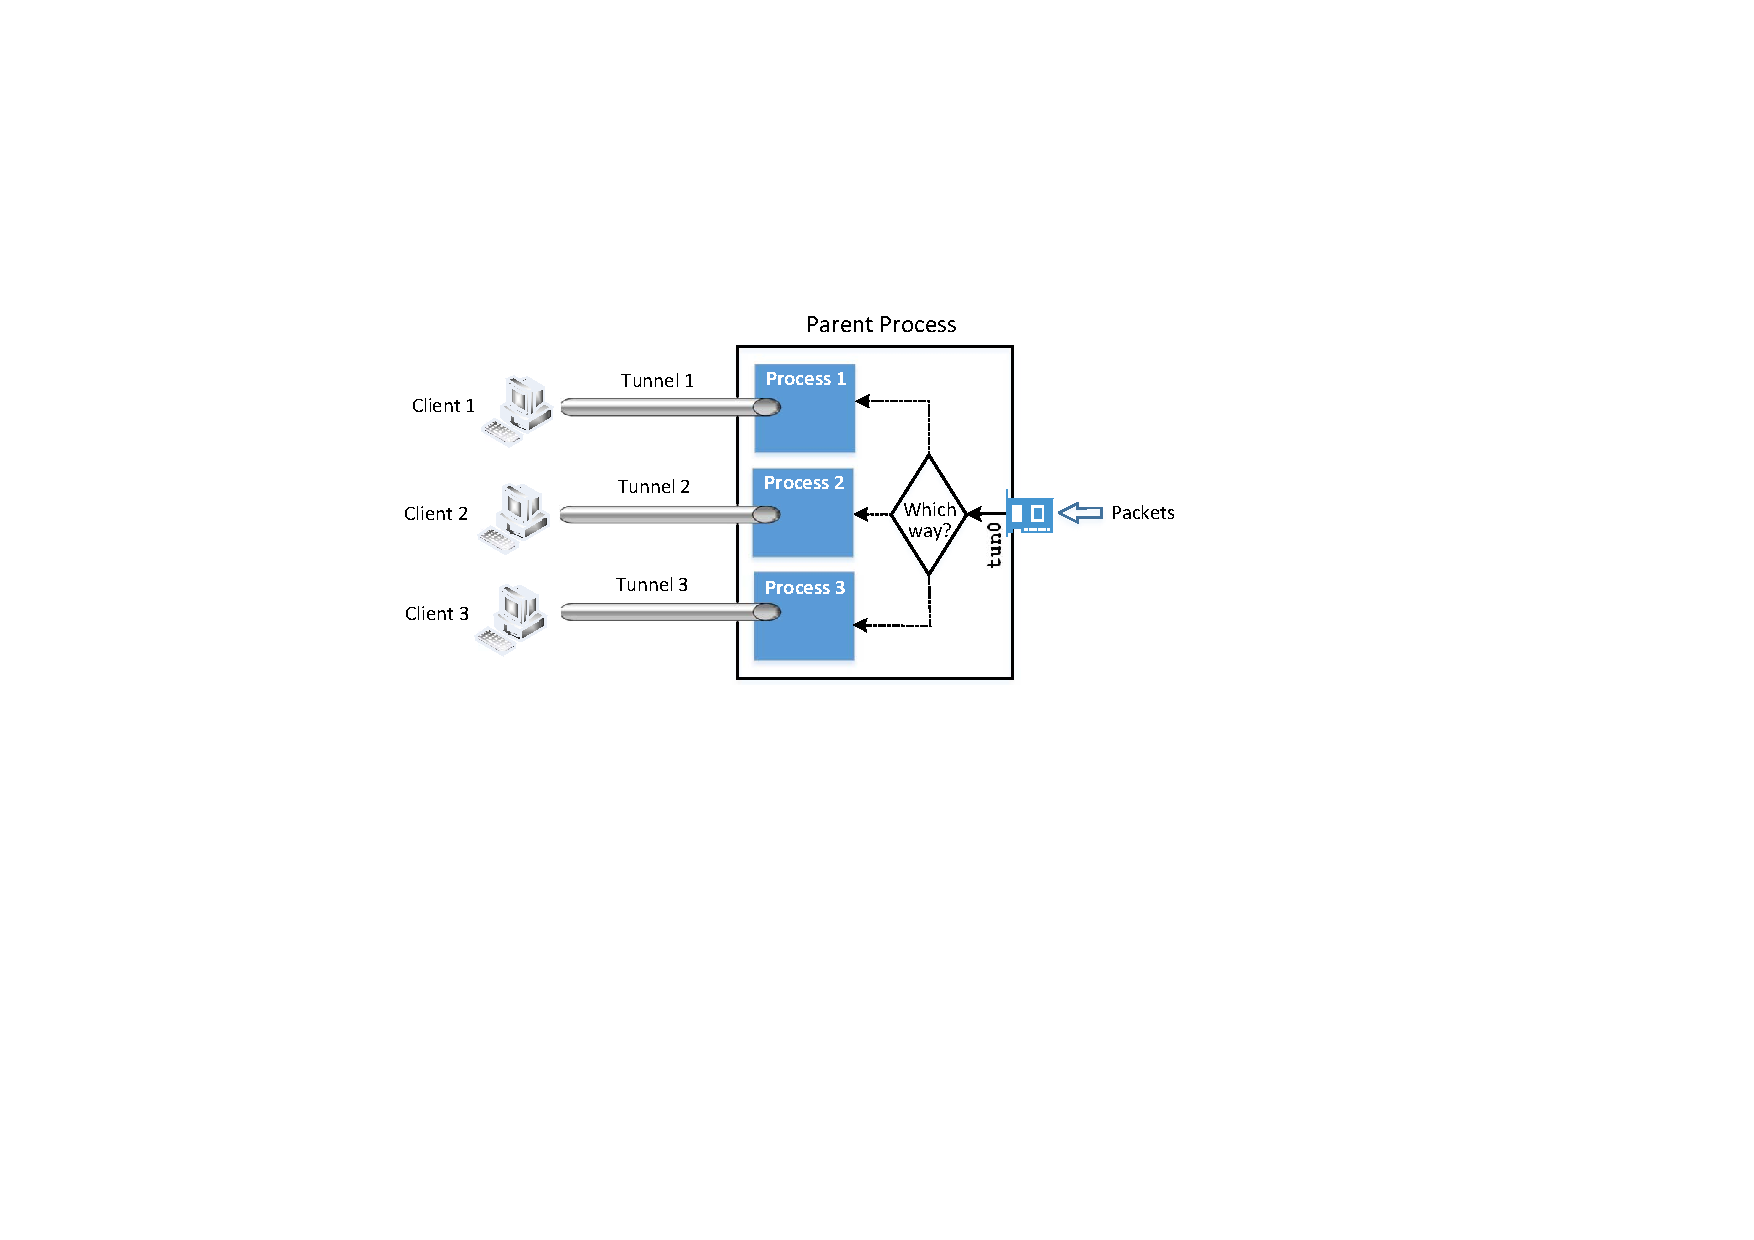
\includegraphics[width=0.8\textwidth]{\vpnFigs/MultiClient.pdf}
\end{center}
\caption{Múltiples clientes en una VPN}
\label{vpn:fig:MultiClient}
\end{figure}
 
En una implementación típica, el proceso servidor VPN (el proceso padre) crea procesos hijos por cada túnel (vea la Figura \ref{vpn:fig:MultiClient}).
Cuando un paquete llega desde el túnel, el proceso hijo que corresponde obtendrá este paquete y lo redirigirá hacia la interfaz TUN.
Esta dirección es la misma sin iomportar si soporta múltiples clientes o no. Es en la otra dirección en donde se convierte en un desafío.
Cuando un paquete llega a la intrefaz TUN (desde la red privada), el proceso padre obtendrá el paquete, y necesitará descubrir a cual túnel este paquete debe de dirigirse. Debe de pensar en como implementar la lógica de esta decisión

Una vez que esta decisión es tomada y se elije un túnel, el proceso padre necesita enviar el paquete al proceso hijo, el cual tiene el túnel que le corresponde. Esto requiere IPC (comunicación entre procesos).
Un enfoque típico es utilizar pipes. Ofrecemos un programa de muestra en la Sección \ref{vpn:subsec: pipe} para mostrar cómo usar pipes para IPC.

Los procesos hijos necesitan monitorear esta interfaz del pipe y leer datos del mismo, si es que los hay. Dado que los procesos hijos también necesitan monitorear los datos que llegan de la interfaz del socket, necesitan estar simultáneamente monitoreando múltiples interfaces.
La Sección \ref{vpn:subsec:select} muestra como hacer esto.


% *******************************************
% SECTION
% ******************************************* 
\section{Guías}


% -------------------------------------------
% SUBSECTION
% ------------------------------------------- 
\subsection{Mostrando Tráfico TLS en Wireshark}

Wireshark identifica el tráfico TLS/SSL basado en los números de puertos. Wireshark sabe que el puerto por defecto para HTTPS es el \texttt{443}, pero nuestro servidor VPN estára a la escucha en un puerto no estandar.
Necesitamos que Wireshark conozca este número de puerto; de otra forma, Wireshark no marcará nuestro tráfico SSL/TLS. Esto es lo que podemos hacer:
Vaya al menú de \texttt{Edit} en Wireshark y elija \texttt{Preferences}, \texttt{Protocols}, \texttt{HTTP}, y vea la entrada que dice \texttt{"SSL/TLS Ports"}. Agregue su puerto SSL en donde su servidor está a la escucha.
Por ejemplo podemos cambiar el contenido de la entrada a \texttt{443,4433}, donde  \texttt{4433} es el puerto usado por nuestro servidor SSL.

\paragraph{Mostrando Tráfico no Cifrado.} El enfoque que se muestra arriba solamente
hace que Wireshark reconozca el tráfico como tráfico TLS/SSL; Wireshark no puede
descifrar el tráfico cifrado. Para fines de depuración, nos gustaría ver el tráfico descifrado.
Wireshark proporciona tal característica; todo lo que tenemos que hacer es proporcionar la clave privada del servidor a Wireshark, y Wireshark automáticamente podrá derivar las claves de sesión del protocolo de enlace TLS/SSL y utilizar estas claves para descifrar el tráfico. 
Para proporcionar la clave privada del servidor a Wireshark, haga lo siguiente:

\begin{lstlisting}
 Click Edit -> Preferences -> Protocols -> SSL 
 Find the "RSA key list", and click the Edit button
 Provide the required information about the server, see this example:
      IP Address: 10.0.2.65
      Port:       4433
      Protocol:   ssl
      Key File:   /home/seed/vpn/server-key.pem  (privat key file)
      Password:   deesdees
\end{lstlisting}


% -------------------------------------------
% SUBSECTION
% ------------------------------------------- 
\subsection{Obteniendo una Dirección IP desde un Hostname}
\label{vpn:subsec:hostnametoip}

Dado un hostname, podemos obtener su dirección IP para este nombre.
En nuestro programa de ejemplo \texttt{tlsclient}, usamos la función \texttt{gethostbyname()} para obtener la dirección IP. Sin embargo, esta función es obsoleta porque no soporta IPv6.
Las aplicaciones deberían de usar \texttt{getaddrinfo()} en su lugar. El siguiente ejemplo muestra como usar esta función para obtener la dirección IP.

\begin{lstlisting}
#include <stdio.h>
#include <stdlib.h>
#include <netdb.h>
#include <netinet/in.h>
#include <sys/socket.h>
#include <arpa/inet.h>

struct addrinfo  hints, *result;

int main() {

  hints.ai_family = AF_INET; // AF_INET means IPv4 only addresses

  int error = getaddrinfo("www.example.com", NULL, &hints, &result);
  if (error) {
      fprintf(stderr, "getaddrinfo: %s\n", gai_strerror(error));
      exit(1);
  }

  // The result may contain a list of IP address; we take the first one.
  struct  sockaddr_in*  ip = (struct sockaddr_in *) result->ai_addr;
  printf("IP Address: %s\n", (char *)inet_ntoa(ip->sin_addr));

  freeaddrinfo(result);
  return 0;
}
\end{lstlisting}
 


% -------------------------------------------
% SUBSECTION
% ------------------------------------------- 
\subsection{Autenticando usando el Archivo Shadow}
\label{vpn:subsec:auth}

El siguiente programa muestra como autenticar a un usuario usando la información de su cuenta guardada en el archivo shadow.
El programa usa la función \texttt{getspnam()} para obtener la información de la cuenta del usuario. Después usa \texttt{crypt()} para hashear el password ingresado y ver si coincide con el obtenido desde el archivo shadow. Si el usuario y el password coinciden, el proceso de autenticación será exitoso.

\begin{lstlisting}
#include <stdio.h>
#include <string.h>
#include <shadow.h>
#include <crypt.h>

int login(char *user, char *passwd)
{
    struct spwd *pw;
    char *epasswd;

    pw = getspnam(user);
    if (pw == NULL) {
        return -1;
    }

    printf("Login name: %s\n", pw->sp_namp);
    printf("Passwd    : %s\n", pw->sp_pwdp);

    epasswd = crypt(passwd, pw->sp_pwdp);
    if (strcmp(epasswd, pw->sp_pwdp)) {
        return -1;
    }

    return 1;
}

void main(int argc, char** argv)
{
   if (argc < 3) {
       printf("Please provide a user name and a password\n");
       return;
   }

   int r = login(argv[1], argv[2]);
   printf("Result: %d\n", r);
}
\end{lstlisting}

Podemos compilar el código anterior y ejecutarlo con un usuario y un password.
Hay que señalar que es necesario contar con privilegios de root a la hora de leer el archivo shadow. Los siguientes comandos indican como compilar y ejecutar el programa.

\begin{lstlisting}
$ gcc login.c -lcrypt
$ sudo ./a.out seed dees
\end{lstlisting}
 
Por último debemos de notar que usamos \texttt{-lcrypt} en la compilación anterior; usamos \texttt{-lcrypto} a la hora de compilar nuestros programas TLS; \texttt{crypt} y \texttt{crypto} son dos librerías diferentes, por lo que esto no es un error de tipeo.


\vspace{0.2in}
% -------------------------------------------
% SUBSECTION
% ------------------------------------------- 
\subsection{Comunicación entre Procesos usando Pipes}
\label{vpn:subsec:pipe}

El siguiente programa muetra como un proceso padre envía datos a su hijo usando pipe. El proceso padre crea un pipe usando  \texttt{pipe()} Línea \ding{192}. 
Cada pipe tiene dos extremos; el primer extremo corresponde al descriptor de archivo de input \texttt{fd[0]}, y el segundo extremo corresponde al descriptor de archivo de output \texttt{fd[1]}.

Después de la creación del pipe, el proceso hijo es lanzado usando \texttt{fork()}. 
Tanto el padre como el hijo tienen descriptores de archivo asociados al pipe. Ellos pueden enviarse datos entre sí usando el pipe, que es bidireccional. Sin embargo, solamente usaremos este pipe para enviar data del padre al hijo y el padre no leerá nada desde el pipe, por lo que cerraremos el extremo del input \texttt{fd[0]} en el proceso padre. De manera similar, el hijo no enviará nada por el pipe, por lo que cerraremos el extremo del output \texttt{fd[1]}. 
En este punto, ya hemos establecido el pipe unidireccional desde el proceso padre hacia su hijo.
Para enviar datos por el pipe, el proceso padre escribe en \texttt{fd[1]} (Línea \ding{193}); para recibir los datos del pipe, el proceso hijo lee desde \texttt{fd[0]} (Línea \ding{194}).  


\begin{lstlisting}
#include <stdio.h>
#include <stdlib.h>
#include <unistd.h>
#include <string.h>

int main(void)
{
  int     fd[2], nbytes;
  pid_t   pid;
  char    string[] = "Hello, world!\n";
  char    readbuffer[80];

  pipe(fd);                                                  (*@\ding{192}@*)
        
  if((pid = fork()) == -1) {
       perror("fork");
       exit(1);
  }

  if(pid>0) { //parent process 
       close(fd[0]); // Close the input end of the pipe. 

       // Write data to the pipe.
       write(fd[1], string, (strlen(string)+1));             (*@\ding{193}@*)
       exit(0);
  }
  else { //child process
       close(fd[1]); // Close the output end of the pipe.

       // Read data from the pipe.
       nbytes = read(fd[0], readbuffer, sizeof(readbuffer)); (*@\ding{194}@*)
       printf("Child process received string: %s", readbuffer);
  }
  return(0);
}
\end{lstlisting}
 



% -------------------------------------------
% SUBSECTION
% ------------------------------------------- 
\subsection{Usando \texttt{select} para Monitorear Múltiples Interfaces}
\label{vpn:subsec:select}

Nuestro programa VPN necesita monitorear múltiples interfaces, incluyendo la interfaz TUN, la interfaz socket y por momentos la interfaz del pipe.
Todas estas interfaces son representadas por descriptores de archivo, por lo que necesitamos monitorearlos para ver si hay data que provienen desde ellos.
Una forma de hacerlo es hacer polling sobre ellos y ver cuando hay datos en cada una de las interfaces. El problema con esta estrategia es que provee una performance poco deseable, porque el proceso debe de seguir de corriendo en un loop infinito aún cuando este ocioso y no haya datos, esto deviene en un gasto de tiempo de procesamiento en el CPU que es innecesario. La otra estrategia es leer desde una interfaz. Por defecto, la lectura es bloqueante es decir el proceso se suspenderá si no hay datos. Cuando los datos esten presentes, el proceso se desbloqueará, y continuará su ejecución. De esta forma, no gastaremos tiempo de CPU cuando no haya datos.

El mecanismo de la lectura bloqueante funciona bien para una interfaz. Si el proceso está a la espera en múltiples intrefaces, no puede bloquearse en una sola, debe de bloquearse en todas las interfaces al mismo tiempo. \linux tiene una llamada al sistema llamada \texttt{select()}, la cual le permite a un programa monitorear múltiples descriptores de archivo al mismo tiempo.
Para usar \texttt{select()}, necesitamos guardar todos los descriptores de archivo que van a ser monitoreados en un conjunto usando la macro \texttt{FD\_SET} (Línea \ding{192} y \ding{193}, en el código que se muestra más abajo), esto bloqueará al proceso hasta que los datos esten disponibles en alguno de los descriptores de archivo del conjunto. Podemos usar la macro \texttt{FD\_ISSET} para ver cual descriptor de archivo es el que ha recibido los datos. En el siguiente ejemplo, usamos \texttt{select()} para monitorear a \texttt{TUN} y el descriptor de archivo de un socket.

\begin{lstlisting}
fd_set readFDSet;
int ret, sockfd, tunfd;

FD_ZERO(&readFDSet);
FD_SET(sockfd, &readFDSet);                                (*@\ding{192}@*)
FD_SET(tunfd, &readFDSet);                                 (*@\ding{193}@*)
ret = select(FD_SETSIZE, &readFDSet, NULL, NULL, NULL);    (*@\ding{194}@*)

if (FD_ISSET(sockfd, &readFDSet){
        // Read data from sockfd, and do something.
}

if (FD_ISSET(tunfd, &readFDSet){
        // Read data from tunfd, and do something. 
}
\end{lstlisting}



% -------------------------------------------
% SUBSECTION
% ------------------------------------------- 
\subsection{Un Ejemplo: usando {\tt telnet} en nuestra VPN} 

Para ayudarlo a entender como fluyen los paquetes desde la aplicación hacia su destino a través de nuestra \miniVPN, hemos dibujado dos figuras para ilustrar el flujo del paquete cuando los usuarios ejecutan  {\tt telnet 10.0.20.100} desde la máquina host, el cual es el Punto A de un host-to-gateway VPNJ. El otro extremo de la VPN es el gateway, el cual está conectado a la red {\tt 10.0.20.0/24}  donde nuestro servidor  {\tt telnet} {\tt 10.0.20.100} reside.

La Figura \ref{fig:example1_host_2_gateway} muestra el flujo del paquete desde el cliente {\tt telnet} hacia el servidor.
La Figura \ref{fig:example2_host_2_gateway}  mmuestra el flujo del paquete desde el servidor {\tt telnet} de regreso hacia el cliente
Solamente describiremos el camino en la Figura \ref{fig:example1_host_2_gateway}. La Figura \ref{fig:example2_host_2_gateway} que muestra el camino de regreso se explica por sí sóla una vez que haya comprendido la Figura \ref{fig:example1_host_2_gateway}.  

\begin{enumerate}

\item Los datos del paquete empiezan desde el programa {\tt telnet}.

\item El kernel construirá un paquete IP con la dirección IP de destino {\tt 10.0.20.100}. 

\item El kernel necesitará decidir cual será la interfaz de red en la cual enrutará el paquete: {\tt eth1} o {\tt tun0}. Necesita configurar su tabla de enrutamiento de manera correcta para que el kernel elija {\tt tun0}. 
Una vez que la decisión es tomada por parte del kernel, este establecerá la dirección IP de origen del paquete usando la dirección IP de la interfaz de red la cual es {\tt 10.0.4.1}.

\item El paquete llegará a nuestro programa VPN (Punto A) a través de la interfaz virtual {\tt tun0}, luego será encriptado y enviado de regreso al kernel a través de un puerto UDP (no a través de la interfaz {\tt tun0}).
Esto es porque nuestro programa VPN usa UDP como nuestro túnel.

\item El kernel tratará al paquete IP encriptado como un dato UDP, construirá un nuevo paquete IP y pondrá todo el paquete IP ya encriptado como el payload del UDP. La nueva dirección IP de destino será el otro extremo del túnel (esto es decidido por el programa VPN que hemos escrito); en la figura, la dirección IP de destino es {\tt 128.230.208.97}.

\item Necesita configurar su tabla de enrutamiento de manera correcta, para que el nuevo paquete sea enrutado por la interfaz  {\tt eth1}; ademas, la dirección IP de origen de este nuevo paquete debería de ser {\tt 209.164.131.32}.

\item El paquete viajará a través de la Internet, junto con el paquete {\tt telnet} original totalmente encriptado y llevado como payload de ese paquete. Esto es el porque del nombre de {\em túnel}.

\item El paquete llegará a nuestro gateway  {\tt 128.230.208.97} a través de su interfaz {\tt eth1}.

\item El kernel le dará el payload UDP (es decir el paquete IP encriptado) al programa VPN (Punto B) que está a a espera de datos UDP por medio de su puerto UDP.

\item El programa VPN desencriptará el payload y lo enviará de regreso al kernel usando la interfaz de red virtual {\tt tun0}.

\item Dado que el paquete viene a través de una interfaz de red, el kernel lo tratará como un paquete IP (bueno en realidad es un paquete IP), mire en su dirección IP de destino y decida por donde enrutarlo. Recuerde, la dirección IP de destino del paquete es {\tt 10.0.20.100}. Si su tabla de enrutamiento está configurada de forma correcta, el paquete debería de ser enrutado por la interfaz {\tt eth2}, porque esta es la interfaz que conecta a la red  {\tt 10.0.20.0/24}.

\item El paquete {\tt telnet} será entregado a su destino final {\tt 10.0.20.100}.

\end{enumerate}

\begin{figure*}
\centering
\begin{tabular}[t]{c}
\subfigure[Un ejemplo del flujo de un paquete desde el cliente elnet hacia el servidor en el Túnel Host-to-Gateway]
{
   \label{fig:example1_host_2_gateway}
   \includegraphics*[viewport=0.7in 1.7in 8.7in 7.3in,width=6.0in]{\vpnFigs/vpn_h2g_details.pdf}
}
\\
\subfigure[Un ejemplo del flujo de un paquete desde el servidor de telnet hacia el cliente en el Túnel Host-to-Gateway]
{
    \label{fig:example2_host_2_gateway}
    \includegraphics*[viewport=1.6in 1.6in 9.6in 7.2in,width=6.0in]{\vpnFigs/vpn_h2g_details_reply.pdf}
}
\end{tabular}
\caption{Ejemplo del Flujo de un Paquete en la VPN.}
\label{fig:example_packetflow}
\end{figure*}





% *******************************************
% SECTION
% ******************************************* 
\section{Informe del Laboratorio y Demostraciones}


%\section*{Submission and Demonstration}


You should submit a detailed lab report to describe your design and implementation.
You should also describe how you test the functionalities and
security of your system. You also need to demonstrate your system to us. 
Please sign up a demonstration time slot with the TA. Please take
the following into consideration when you prepare for demonstraiton:

\begin{itemize}

\item The total time of the demo will be 15 minutes, no more additional time would be
given. So prepare your demonstration so you can cover the important features.  

\item You are entirely responsible for showing the demo. 
We will NOT even touch the keyboard during the
demonstration; so you should not depend on us to test your system. If you fail to demo
some important features of your system, we will assume that your system does not
have those features. 

\item You need to practice before you come to the demonstration. 
If the system crashes or anything goes wrong, it is your own fault. We will not 
debug your problems, nor give you extra time for it. 

\item 
During the demo, you should consider yourself as salesmen, and you want to sell
your system to us. You are given 15 minutes to show us how good your system is.
So think about your sales strategies. If you have implemented a great system,
but fail to show us how good it is, you are not likely to get a good grade. 

\item 
Do turn off the messages your system prints out for debugging purposes. 
Those messages should not appear in a demonstration.


\end{itemize}






% *******************************************
% SECTION
% ******************************************* 
\section{Checklist de la Demostración}

Durante el período de pandemia COVID-19, no hemos podido hacer las demostraciones en personas. Sin embargo hacerlas online es una opción, hemos decidido experimentar con un método diferente: pidiendóle a los estudiantes que graben su demostración y envién el archivo de video. Para ayudarlos a realizar su propía guía para la demostración, hemos provisto una serie de checks en una lista en la Tabla \ref{vpn:table:checklist}. Incluso si se realiza esta demostración en persona, este checklist es útil.


\renewcommand{\arraystretch}{1.5}

\begin{longtable}{|p{0.3\textwidth}|p{0.7\textwidth}|}
 \caption{Checklist para la demostración VPN}
 \label{vpn:table:checklist}
 \endfirsthead
 \endhead
 \hline\xrowht[()]{10pt}
 \textbf{\Large Requerimientos} & \textbf{\Large Detalles} \\ 
 \hline
 \hline
 \textbf{Estado Inicial} & 
	\vspace*{-0.3cm}
 	\begin{itemize}[topsep=-0.5cm,leftmargin=0.4cm]
 		\item Reinicie las trés Máquinas Virtuales. Empiece la grabación después de que las Máquinas Virtuales sean reiniciadas. Debería de comenzar la demostración inmediatamente después de que hayan sido reiniciadas. Si espera demasiado, tendrá que hacer los reinicios nuevamente.
 		
		\item Escriba en la terminal \texttt{"last reboot; date"}  para mostrar el tiempo de reinicio y el tiempo actual de cada una de las tres máquinas virtuales. La diferencia entre estos dos tiempos no debería de ser más de 5 minutos.

		\item Muestre las tablas de enrutamiento en las tres máquinas virtuales.
	\end{itemize}
 \\ 
 \hline
 
 \textbf{Testeo Pre-Túnel} & 
 	\vspace*{-0.3cm}
 	\begin{itemize}[topsep=-0.5cm,leftmargin=0.4cm]
 		\item Antes de hacer el setup de la VPN, haga un \texttt{ping} al Host \hostv desde el Host \hostu y explique sus observaciones.
	\end{itemize}
 \\ 
 \hline

 \textbf{Creación del Túnel} & 
 	\vspace*{-0.3cm}
 	\begin{itemize}[topsep=-0.5cm,leftmargin=0.4cm]
	   \item Corra su cliente VPN y su servidor VPN.
		\begin{itemize}
		\item Necesita de tipear los passwords para autenticarse en el servidor, el password no debería de ser visible (se descontarán 10 puntos si vemos sus passwords). Puede usar \texttt{getpass()} para lograr este objetivo (para ver el manual use  ``\texttt{man getpass}")
		
		\item Los passwords no pueden ser hardcodeados en su programa. Si lo hace, se le descontarán 50 puntos.
		\end{itemize}

	   \item Realice esta configuración en todas las máquinas virtuales. Aunque puede poner los comandos de configuración en un script, necesita mostrar el script y explicar los comandos de su script.

	   \item  Muestre las tablas de enrutamiento en las tres máquinas virtuals después de la configuración.
	\end{itemize}
 \\ 
 \hline

 \textbf{Testeo del Ping} & 
 	\vspace*{-0.3cm}
 	\begin{itemize}[topsep=-0.5cm,leftmargin=0.4cm]
 		\item En el Host \hostu: realize un \texttt{ping} al Host \hostv.
		\item Use Wireshark para demostrar que su VPN funciona bien.
		\item Muestrenos la prueba de que el túnel está encriptado.
	\end{itemize}
 \\ 
 \hline

 \textbf{Testeo del Telnet} & 
 	\vspace*{-0.3cm}
 	\begin{itemize}[topsep=-0.5cm,leftmargin=0.4cm]
		\item En el Host \hostu: haga \texttt{telnet} al Host \hostv.
		\item Use Wireshark para demostrar que su VPN funciona bien.
	\end{itemize}
 \\ 
 \hline

 \textbf{Testeo del Tunnel-Breaking} & 
 	\vspace*{-0.3cm}
 	\begin{itemize}[topsep=-0.5cm,leftmargin=0.4cm]
 		\item En el Host \hostu, haga un telnet al Host \hostv. Mientras que la conexión telnet corte el túnel VPN parando el cliente vpn y el/los servidor/es vpns.
 		Escriba algo en la ventana de telnet. ¿Puede ver lo que tipea? ¿Qué ocurre con la conexión TCP? ¿Se corta la conexión?

		\item Vamos a reconectar nuestro túnel VPN (no espere mucho tiempo). Ejecute nuevamente los programas cliente y servidore y realize las configuraciones necesarias. Una vez que el túnel se reestableció, fijese que pasa con la conexión telnet, por favor explique y describa su observación.
	\end{itemize}
 \\ 
 \hline

 \textbf{Testeo de Paquete Grande} & 
 	\vspace*{-0.3cm}
 	\begin{itemize}[topsep=-0.5cm,leftmargin=0.4cm]
 	\item Envíe un paquete grande (tamaño \textgreater\space 3000) desde el Host \hostu al Host \hostv. Puede usar \texttt{"ping -s"} para hacerlo.

	\item Use Wireshark explique y describa su observación.
	\end{itemize}
 \\ 
 \hline

 \textbf{Setup de TLS} & 
 	\vspace*{-0.3cm}
 	\begin{itemize}[topsep=-0.5cm,leftmargin=0.4cm]
 		\item Muestrenos como ha configurado su TLS en el cliente y en el servidor.
 		\item Muestrenos en donde ha ubicado los certificados para el servidor y los certificados autofirmados.
 		\item Muestrenos que líneas de código cargan esos certificados.
	\end{itemize}
 \\ 
 \hline

 \textbf{Testeo de MITM} & 
 	\vspace*{-0.3cm}
 	\begin{itemize}[topsep=-0.5cm,leftmargin=0.4cm]
 		\item Demuestre que su sistema puede derrotar con éxito ataques MITM. Necesita simular un ataque MITM y demostrar que su programa cliente puede derrotarlo.
	\end{itemize}
 \\ 
 \hline

 \textbf{Explicación del Código 1} & 
	Cualés son las líneas de código responsables de lo siguiente:
 	\vspace*{0.2cm}
 	\begin{itemize}[topsep=-0.5cm,leftmargin=0.4cm]
 		\item Verificar que el certificado del servidor sea válido
 		\item Verificar que el servidor es el dueño del certificado
 		\item Verificar que el servidor es el servidor indicado
	\end{itemize}
 \\ 
 \hline

 \textbf{Explicación del Código 2} & 
 	Cual es la línea del código en el programa cliente que fuerza el handshake TLS que detiene el proceso si la verificación del certificado del servidor falla?
 \\ 
 \hline

 \textbf{Explicación del Código 3} & 
	Que línea(s) del código es responsable de lo siguiente:
	\vspace*{0.2cm}
 	\begin{itemize}[topsep=-0.5cm,leftmargin=0.4cm]
 		\item Enviar el usuario y password al servidor
 		\item Obtener la información de la cuenta de usuario en el archivo shadow
	\end{itemize}
 \\ 
 \hline

 \textbf{Tiempo Final} & 
	Escriba los comandos \texttt{"last reboot; date"} para mostrar el tiempo antes de terminar su demostración.
 \\ 
 \hline

\end{longtable}



\section*{Agradecimientos}

Este documento ha sido traducido al Español por Facundo Fontana



\end{document}


